\section{Analysis}
\label{sec:analysis}

\subsection{Controllability: The $\gamma$ Curve}

Figure~\ref{fig:gamma_curve} plots key metrics as a function of $\gamma$ for \styleshield{} and the two strongest baselines.
Several observations emerge:

\textbf{Monotonic controllability.}
As $\gamma$ increases from 5.0 to 7.0, $\pai$ on Det-v3 decreases monotonically from 0.703 to 0.130 (an 81.5\% relative reduction), while semantic similarity decreases gracefully from 0.948 to 0.928 (only 2.1\% relative loss).
This confirms that $\gamma$ serves as a reliable, continuous control knob for the evasion--preservation trade-off.

\textbf{Pareto dominance.}
At every operating point along the $\gamma$ curve, \styleshield{} Pareto-dominates Backtranslation: at comparable evasion levels (e.g., ${\sim}$82\%), \styleshield{} achieves substantially higher semantic similarity (0.942 at $\gamma{=}6.0$ vs.\ 0.852 for Backtranslation).
The Synonym and LLM Rewrite baselines are confined to the high-$\pai$ region and cannot reach meaningful evasion at any quality level.

\textbf{Cross-detector consistency.}
On unseen detectors, the $\gamma$ curve is even more favorable: at $\gamma{=}6.0$, \styleshield{} already achieves $>$92\% evasion on all three unseen detectors (ANX-BERT, Det-v2, GPT2-Det), while maintaining 0.942 semantic similarity.

\begin{figure}[t]
    \centering
    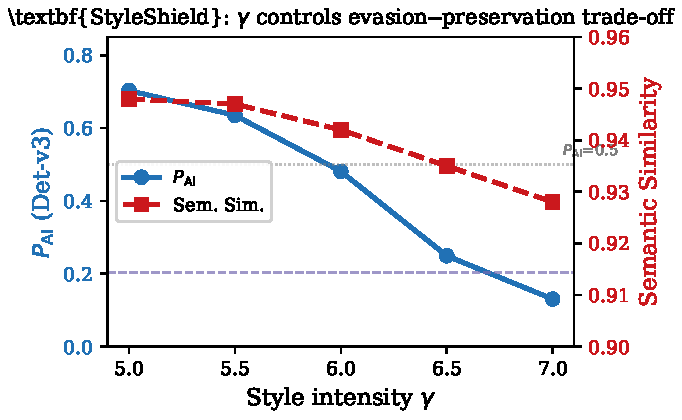
\includegraphics[width=\columnwidth]{figures/fig2_gamma_curve.pdf}
    \caption{$\pai$ (solid) and semantic similarity (dashed) as functions of $\gamma$ on Det-v3. The backtranslation baseline's $\pai$ is shown as a dashed reference line. \styleshield{} provides smooth, monotonic control; the ``sweet spot'' lies around $\gamma{=}6.5$--$7.0$.}
    \label{fig:gamma_curve}
\end{figure}

\begin{figure}[t]
    \centering
    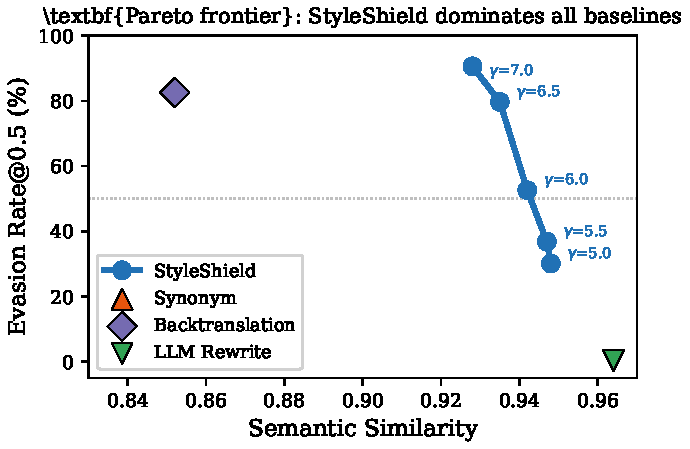
\includegraphics[width=\columnwidth]{figures/fig3_pareto.pdf}
    \caption{Pareto frontier of evasion rate vs.\ semantic similarity. \styleshield{} traces a smooth curve that Pareto-dominates all baselines: at any given similarity level, it achieves higher evasion, and vice versa.}
    \label{fig:pareto}
\end{figure}

\subsection{Perplexity Analysis}

An initially counterintuitive finding is that \styleshield{}'s output PPL (${\sim}$21) exceeds that of human text (${\sim}$16.5), which in turn exceeds original AI text (${\sim}$10.7).
We argue this pattern is \emph{desirable}: low PPL is precisely the statistical regularity that detectors exploit.
AI-generated text is ``too perfect''---it follows high-probability paths through the language model's distribution, resulting in low perplexity.
Human text, by contrast, contains idiosyncratic word choices, colloquialisms, and stylistic variation that increase perplexity.
\styleshield{}'s elevated PPL reflects successful injection of human-like variability, pushing the text's statistical profile beyond the narrow AI distribution.

The ablation with shallow Qwen features (A3, layer 7) exhibits extreme PPL (99.9--106.9), indicating that without strong semantic grounding, the model introduces \emph{too much} variation, degrading fluency.
The full model with layer-14 features achieves the right balance: enough variation to evade detection (PPL$\approx$21) while remaining within the range of fluent text.

\subsection{What Does the Detector Reward Actually Do?}

The A1 ablation (no detector reward) achieves \emph{better} evasion than the full model at every $\gamma$ (e.g., 95.4\% vs.\ 90.6\% at $\gamma{=}7.0$).
At first glance, this seems to argue against including the detector reward.
However, the quality metrics tell a different story: without the reward, PPL increases to 26.1--26.4 (vs.\ 21.1--21.2), and semantic similarity drops to 0.921 (vs.\ 0.928).

We hypothesize that the detector reward acts as an \emph{implicit quality regularizer}: by providing a gradient signal specifically for detection evasion, it allows the base CE loss to focus more on reconstruction quality rather than ``accidentally'' achieving evasion through content distortion.
In other words, the detector reward teaches the model to evade \emph{efficiently}---achieving strong evasion with minimal collateral damage to text quality.
